% Setup -------------------------------

\documentclass[a4paper]{report}
\usepackage[a4paper, total={6in, 10in}]{geometry}
\setcounter{secnumdepth}{3}
\setcounter{tocdepth}{3}

\usepackage{titlepic}

\usepackage{hyperref}
\usepackage{indentfirst}

\usepackage{graphicx}
\usepackage{float}

\usepackage{enumitem}

\usepackage{minted}
\usepackage{xcolor}

\definecolor{friendlybg}{HTML}{f0f0f0}
\setminted[bash]{
	style=manni,
	bgcolor=friendlybg,
	linenos,
	frame=lines,
	framerule=0.6pt,
	framesep=5pt,
	rulecolor=orange,
	fontsize=\footnotesize
}
\setminted[dockerfile]{
	style=manni,
	bgcolor=friendlybg,
	linenos,
	frame=lines,
	framerule=0.6pt,
	framesep=5pt,
	rulecolor=orange,
	fontsize=\footnotesize
}

% Encoding
%--------------------------------------
\usepackage[T1]{fontenc}
\usepackage[utf8]{inputenc}
%--------------------------------------

% Portuguese-specific commands
%--------------------------------------
\usepackage[portuguese]{babel}
%--------------------------------------

% Hyphenation rules
%--------------------------------------
\usepackage{hyphenat}
%--------------------------------------

% Capa do relatório

\title{
    Gestão de Grandes Conjuntos de Dados
    \\ \Large{\textbf{2º Trabalho Prático}}
    \\ -
    \\ Mestrado em Engenharia Informática
    \\ Universidade do Minho
}
\author{
    \begin{tabular}{ll}
        \textbf{Grupo nº 8}
        \\
        \hline
        PG41080 & João Ribeiro Imperadeiro
        \\
        PG41081 & José Alberto Martins Boticas
        \\
        PG41091 & Nelson José Dias Teixeira
        \\
        PG41851 & Rui Miguel da Costa Meira
    \end{tabular}
    \vspace{1cm}
}

\date{\today}

\titlepic{
	\vspace{2cm}
	
\includegraphics[scale=0.065]{Imagens//EEUM_logo.png}
}

\begin{document}

\begin{titlepage}
    \maketitle
\end{titlepage}

% Índice

\tableofcontents
\listoffigures

% Introdução

\chapter{Introdução} \label{ch:Introduction}
\large {
    Neste trabalho prático é requerida a concretização e avaliação experimental de tarefas de armazenamento e processamento de dados através do uso da ferramenta computacional \textit{Spark} (\textit{batch} e \textit{streaming}).
    Por forma a realizar estas tarefas, são utilizados os dados públicos do \textit{IMDb}, que se encontram disponíveis em:
    \begin{center}
        \textit{\url{https://www.imdb.com/interfaces/}}
    \end{center}

    Para além destes dados, é também utilizado um gerador de \textit{streams}, baseado nos mesmos, que simula uma sequência de votos individuais de utilizadores. Este utensílio foi desenvolvido pelo docente desta unidade curricular e encontra-se disponível na plataforma \textit{Blackboard}.

    Ao longo deste documento vão também ser expostos todos os passos tomados durante a implementação das tarefas pedidas neste projeto, incluindo as decisões tomadas pelos elementos deste grupo a nível de algoritmos e parâmetros de configuração.
    Para além disso são ainda apresentadas todas as instruções que permitem executar e utilizar corretamente os programas desenvolvidos.
    Por fim, na fase final deste manuscrito, são exibidos os objetivos atingidos após a realização das tarefas propostas.

    De salientar também que durante os capítulos que se seguem são identificadas algumas alternativas para concretizar as tarefas indicadas neste trabalho prático.	
}

\chapter{Implementação} \label{ch:Implementation}
\large {
    Para a realização com sucesso deste trabalho prático, é solicitada a elaboração de três tarefas. Apresentam-se de seguida as mesmas:
    \begin{enumerate}
        \item Desenvolver uma componente de processamento de \textit{streams} que produza os seguintes resultados:
        \begin{itemize}
            \item \textbf{\textit{Log}}: armazenar todos os votos individuais recebidos, etiquetados com a hora de chegada aproximada ao minuto, em lotes de 10 minutos. Cada lote deve ser guardado num ficheiro cujo nome identifica o período de tempo;
            \item \textbf{\textit{Top3}}: exibir a cada minuto o \textit{top} 3 dos títulos que obtiveram melhor classificação média nos últimos 10 minutos;
            \item \textbf{\textit{Trending}}: apresentar a cada 15 minutos os títulos em que o número de votos recolhido nesse período sejam superiores aos votos obtidos no período anterior, independentemente do valor dos votos.
        \end{itemize}
        \item Implementar uma componente de processamento em \textit{batch} que permita realizar as seguintes tarefas:
        \begin{itemize}
            \item \textbf{\textit{Top10}}: calcular o \textit{top} 10 dos atores que participaram em mais títulos diferentes;
            \item \textbf{\textit{Friends}}: computar o conjunto de colaboradores de cada ator (i.e., outros atores que participaram nos mesmos títulos);
            \item \textbf{\textit{Ratings}}: atualizar o ficheiro \textsl{"title.ratings.tsv"} tendo em conta o seu conteúdo anterior e os novos votos recebidos até ao momento.
        \end{itemize}
        \item Escolher a configuração e a implementação que, para o mesmo \textit{hardware}, permite receber e tratar o maior débito de eventos. Esta tomada de decisão deve ser devidamente justificada com recurso a resultados experimentais.
    \end{enumerate}
    
    Nas próximas secções são evidenciadas as implementações para cada uma destas tarefas bem como algumas sugestões alternativas que poderiam ser tomadas em consideração.

    \section{Configuração} \label{sec:Configuration}
        Nesta secção do relatório são apresentadas as configurações relativas ao arranque do \textit{cluster}, instanciando-se tanto as respetivas entidades (\textsl{master}, \textsl{worker1} e \textsl{worker2}) como as máquinas virtuais pertencentes à plataforma \textit{Google Cloud}, e, ainda, a configuração genérica para a execução individual de cada exercício proposto. 

        \subsection{Arranque do \textit{cluster}}
            A configuração escolhida para a realização deste projeto coincide com a que foi sugerida pelo docente desta unidade curricular, isto é, o \textbf{\textit{docker swarm}}.
            Esta configuração permite não só tirar partido da ferramenta computacional \textit{Google Cloud} como também possibilita o uso de plataformas como o \textit{Hadoop HDFS} e o \textit{Apache Spark}.
            Como seria de esperar, todos os ficheiros de \textit{input} utilizados para atingir os objetivos traçados neste trabalho prático são armazenados no sistema \textit{Hadoop HDFS}.
            
            Exibe-se de seguida todos os passos de configuração associados ao \textit{docker swarm}:
            \begin{enumerate}[label=\textbf{\arabic*.}]
                \item criação das instâncias relativas às 3 entidades intrínsecas à arquitetura do sistema, isto é, as entidades \textsl{master}, \textsl{worker1} e \textsl{worker2}:
                \begin{figure}[H]
                    \centering
                    \begin{minted}{bash}
docker-machine create \
               --driver google --google-project ferrous-aleph-271712 \
               --google-zone europe-west1-b \
               --google-machine-type n1-standard-2 \
               --google-disk-size=100 \
               --google-disk-type=pd-ssd \
               --google-machine-image \
       https://www.googleapis.com/compute/v1/projects/centos-cloud/global/images/centos-7-v20200309 \
               master
                    \end{minted}
                    \vspace{-5mm}
                    \caption{Configuração - Criação da instância associada à entidade \textsl{master}}
                    \label{fig:1}
                \end{figure}
                
                \begin{figure}[H]
                    \centering
                    \begin{minted}{bash}
docker-machine create \
               --driver google --google-project ferrous-aleph-271712 \
               --google-zone europe-west1-b \
               --google-machine-type n1-standard-2 \
               --google-disk-size=100 \
               --google-disk-type=pd-ssd \
               --google-machine-image \
       https://www.googleapis.com/compute/v1/projects/centos-cloud/global/images/centos-7-v20200309 \
               worker1
                    \end{minted}
                    \vspace{-5mm}
                    \caption{Configuração - Criação da instância associada à entidade \textsl{worker1}}
                    \label{fig:2}
                \end{figure}

                \begin{figure}[H]
                    \centering
                    \begin{minted}{bash}
docker-machine create \
               --driver google --google-project ferrous-aleph-271712 \
               --google-zone europe-west1-b \
               --google-machine-type n1-standard-2 \
               --google-disk-size=100 \
               --google-disk-type=pd-ssd \
               --google-machine-image \
       https://www.googleapis.com/compute/v1/projects/centos-cloud/global/images/centos-7-v20200309 \
               worker2
                    \end{minted}
                    \vspace{-5mm}
                    \caption{Configuração - Criação da instância associada à entidade \textsl{worker2}}
                    \label{fig:3}
                \end{figure}

                De salientar que a designação \texttt{ferrous-aleph-271712} corresponde ao identificador do projeto presente na plataforma \textit{Google Cloud} de um dos elementos que compõem este grupo.
                Assim, esta denominação deve ser substituída pelo nome do projeto do utilizador em causa.

                \item configuração do \textit{swarm} relativo às entidades \textsl{master}, \textsl{worker1} e \textsl{worker2}:
                \begin{figure}[H]
                    \centering
                    \begin{minted}{bash}
docker-machine ssh master sudo docker swarm init
                    \end{minted}
                    \vspace{-5mm}
                    \caption{Configuração - \textit{swarm} \textsl{master}}
                    \label{fig:4}
                \end{figure}

                \begin{figure}[H]
                    \centering
                    \begin{minted}{bash}
docker-machine ssh worker1 sudo docker swarm join --token \
               SWMTKN-1-5zfy2iio54tma997pnt96gq5095fimqn2hxr2a8j16ogq0n3c9-0kp6mi5iuj956gpl9sfccd5bo\
               10.132.0.8:2377
                    \end{minted}
                    \vspace{-5mm}
                    \caption{Configuração - \textit{swarm} \textsl{worker1}}
                    \label{fig:5}
                \end{figure}

                \begin{figure}[H]
                    \centering
                    \begin{minted}{bash}
docker-machine ssh worker2 sudo docker swarm join --token \
               SWMTKN-1-5zfy2iio54tma997pnt96gq5095fimqn2hxr2a8j16ogq0n3c9-0kp6mi5iuj956gpl9sfccd5bo\
               10.132.0.8:2377
                    \end{minted}
                    \vspace{-5mm}
                    \caption{Configuração - \textit{swarm} \textsl{worker2}}
                    \label{fig:6}
                \end{figure}

                \item ativação do ambiente da entidade \textsl{master}:
                \begin{figure}[H]
                    \centering
                    \begin{minted}{bash}
docker-machine env master
eval $(docker-machine env master)
                    \end{minted}
                    \vspace{-5mm}
                    \caption{Configuração - Ativação do ambiente da entidade \textsl{master}}
                    \label{fig:7}
                \end{figure}

                \item verificação da existência das 3 entidades presentes no sistema e das respetivas propriedades:
                \begin{figure}[H]
                    \centering
                    \begin{minted}{bash}
docker node ls
                    \end{minted}
                    \vspace{-5mm}
                    \caption{Configuração - Verificação da existência das 3 entidades do sistema}
                    \label{fig:8}
                \end{figure}

                \item compilação do gerador de \textit{streams}, isto é, o \textit{streamgen}:
                \begin{figure}[H]
                    \centering
                    \begin{minted}{bash}
mvn package
docker build -t streamgen .
                    \end{minted}
                    \vspace{-5mm}
                    \caption{Configuração - Compilação d utensílio \textit{streamgen}}
                    \label{fig:9}
                \end{figure}

                \item arranque do sistema com a configuração \textit{swarm} especificada:
                \begin{figure}[H]
                    \centering
                    \begin{minted}{bash}
docker stack deploy -c ../swarm-spark/docker-compose.yml mystack
                    \end{minted}
                    \vspace{-5mm}
                    \caption{Configuração - Arranque do sistema}
                    \label{fig:10}
                \end{figure}

                É de realçar que no ficheiro \textit{"docker-compose.yml"} encontra-se uma configuração \textit{docker} semelhante à que foi utilizada no guião nº 8 desta unidade curricular.
                A única diferença presente no mesmo diz respeito à integração do gerador de \textit{streams} (\textit{streamgen}) desenvolvido pelo docente como um \textit{container docker} do sistema.
                Assim, no momento do arranque do sistema, a ferramenta \textit{streamgen} é convenientemente invocada, ficando à espera de novas conexões por parte dos utilizadores.
                Apresenta-se de seguida a configuração presente no ficheiro \textit{"docker-compose.yml"} relativa ao \textit{streamgen}:

                \begin{figure}[H]
                    \centering
                    \begin{minted}{bash}
streamgen:
    image: streamgen
    command: hdfs:///data/title.ratings.tsv 120
    env_file:
        - ./hadoop.env
    deploy:
        mode: replicated
        replicas: 1
        placement:
            constraints:
                - "node.role==manager"
                    \end{minted}
                    \vspace{-5mm}
                    \caption{Configuração - Ficheiro \textit{"docker-compose.yml"} - \textit{streamgen}}
                    \label{fig:11}
                \end{figure}

                \item verificação da disponibilidade do serviço relativo à rede \textit{mystack\_default}:
                \begin{figure}[H]
                    \centering
                    \begin{minted}{bash}
docker stack ls
docker service ls
docker network ls
                    \end{minted}
                    \vspace{-5mm}
                    \caption{Configuração - Verificação da disponibilidade do serviço relativo à rede \textit{mystack\_default}}
                    \label{fig:12}
                \end{figure}

                \item acesso à plataforma \textit{Hadoop HDFS} por parte do utilizador:
                \begin{figure}[H]
                    \centering
                    \begin{minted}{bash}
docker run --network mystack_default --env-file ../swarm-spark/hadoop.env -it bde2020/hadoop-base \
       bash
                    \end{minted}
                    \vspace{-5mm}
                    \caption{Configuração - Acesso à plataforma \textit{Hadoop HDFS}}
                    \label{fig:13}
                \end{figure}
            \end{enumerate}}

            Com a concretização dos 7 passos descritos acima fica concluída a configuração associada à ferramenta \textit{docker swarm}.
        
        \subsection{Execução de tarefas}
        Para a execução dos 6 exercícios descritos na \hyperref[ch:Implementation]{secção} relativa à implementação, é disponibilizado um ficheiro com a designação \textit{Dockerfile}.
        Neste é especificado o nome da classe relativa à proposta que se presente executar, procedendo corretamente à sua invocação.
        Como tal, em primeiro lugar é preciso desempenhar a seguinte instrução:
        \begin{figure}[H]
            \centering
            \begin{minted}{bash}
mvn package
            \end{minted}
            \vspace{-5mm}
            \caption{Configuração - Obtenção do ficheiro \textit{jar} do projeto}
            \label{fig:14}
        \end{figure}
        
        De seguida, invoca-se o \textit{dockerfile} em causa. Expõe-se agora o seu conteúdo:
        \begin{figure}[H]
            \centering
            \begin{minted}{dockerfile}
FROM bde2020/spark-base:2.4.4-hadoop2.7
COPY target/TP2-1.0-SNAPSHOT.jar /
ENTRYPOINT ["/spark/bin/spark-submit", "--class", "package.className", "--master", \
            "spark://spark-master:7077", "/TP2-1.0-SNAPSHOT.jar"]
            \end{minted}
            \vspace{-5mm}
            \caption{Configuração - \textit{Dockerfile}}
            \label{fig:15}
        \end{figure}

        A este ficheiro estão associadas alguma opções de execução que garantem uma comunicação fidedigna com o sistema inicialmente declarado. Eis as mesmas:
        \begin{figure}[H]
            \centering
            \begin{minted}{bash}
-p 4040:4040 --network mystack_default --env-file ../swarm-spark/hadoop.env
            \end{minted}
            \vspace{-5mm}
            \caption{Configuração - Opções de execução do ficheiro \textit{Dockerfile}}
            \label{fig:16}
        \end{figure}

        De salientar que é escolhida a opção \textsl{master} no campo relativo ao \textit{docker machine} para, mais uma vez, garantir uma configuração válida do sistema em causa.

    \section{1ª Tarefa} \label{sec:Task1}
        Na 1ª tarefa deste projeto é pedido o desenvolvimento de uma componente de processamento de \textit{streams}. Nesta é solicitada a realização de vários exercícios com diferentes caraterísticas. Como tal, apresenta-se de seguida as respetivas implementações e, ainda, possíveis alternativas nas suas concretizações.

        \subsection{\textit{Log}} \label{subsec:Task1-Log}
        Neste exercício, tal como foi indicado anteriormente neste \hyperref[ch:Implementation]{capítulo}, é imposto o armazenamento de todos os votos individuais recebidos com a indicação da hora de chegada aproximada ao minuto, em lotes de 10 minutos, sendo que cada lote é guardado com o nome relativo ao período de tempo em causa.

        Dito isto, para proceder ao tratamento da aproximação da hora recebida ao minuto, foi implementada uma função para o efeito. O grupo optou por não só guardar a hora referida como também a data em questão, exibindo, desta forma, um maior detalhe da informação recebida.
        Uma vez implementada esta função, seguindo a sugestão fornecida pelo docente desta unidade curricular, foi utilizado o método \textit{transform} que faz uso da noção de tempo. Com esta vertente, é possível associar a cada \textit{rdd} do conjunto de dados o tempo exato em que este foi processado.

        Por fim, com os aspetos computacionais mencionados acima, resta armazenar os dados recebidos pela ferramenta \textit{streamgen} com recurso à definição de uma janela que respeite o enunciado deste exercício, isto é, 10 minutos de duração e 10 minutos de deslocamento.
        Os \textit{rdd's} em causa são guardados na diretoria \texttt{Log/Lot\{\textit{i}\} - dd-MM-yyyy HH-mm}, sendo que \texttt{i} diz respeito ao número do lote (que começa no número 1 e que é constamente incrementado) e \texttt{dd-MM-yyyy HH-mm} refere-se ao padrão do período temporal.
        De maneira a coletar num só ficheiro (\textit{part-00000}) todos os \textit{rdd's} referentes a este exercício, foi aplicado o método \textit{coalesce(1)}.
        Esta última função, quando comparada com a \textit{repartition()}, não necessita de efetuar um \textit{shuffle} completo dos dados e, para além disso, é mais otimizada para a redução do número de partições.
        Para além disto, esta abordagem foi considerada nesta implementação dado que no exercício \textit{Ratings} (\textit{batch}) será necessário realizar a leitura do ficheiro mencionado. Consequentemente, em vez de operar várias leituras de ficheiros associados a \textit{rdd's}, efetua-se apenas uma leitura, permitindo, assim, uma maior eficiência.

        \subsection{\textit{Top3}} \label{subsec:Task1-Top3}
            \subsubsection{Alternativa} \label{sssec:Task1-Top3-Alternativa} 

        \subsection{\textit{Trending}} \label{subsec:Task1-Trending}
            \subsubsection{Alternativa} \label{sssec:Task1-Trending-Alternativa}

    \section{2ª Tarefa} \label{sec:Task2}

        \subsection{\textit{Top10}} \label{subsec:Task2-Top10}
            Tal como foi mencionado no início \hyperref[ch:Implementation]{2º capítulo}, nesta subtarefa é pedido o cálculo dos 10 atores que participaram em mais filmes distintos.

            Durante o processamento inicial do ficheiro \textsl{"title.principals.tsv"} é, tal como seria de esperar, ignorado o respetivo cabeçalho.
            Posteriormente, é extraída, linha após linha, a informação pertinente do mesmo, isto é, os identificadores do filme e do ator em questão, agrupando os dados pela segunda componente. Esta última ação é efetuada com recurso à chamada do método \textit{groupByKey}.
            Uma vez realizada esta computação, obtém-se para cada ator a lista de filmes em que este participou. Atendendo ao resultado exigido neste exercício, basta, nesta etapa do processamento, efetuar a contagem dos filmes associados a cada ator, filtrando os 10 registos com maiores valores.

            A recolha dos 10 atores que participaram em mais filmes é formalizada com a chamada do método \textit{top}. Esta função permite extrair os \textit{k} maiores registos de um \textit{RDD} segundo uma determinada ordem.
            Para o caso deste exercício, houve a necessidade de implementar um comparador explícito, numa classe à parte, dado que o tipo de dados \textit{Tuple2} não é, por definição, serializável.

            Tendo em consideração este último detalhe, conclui-se a realização desta subtarefa.

            \begin{figure}[H]
                \centering
                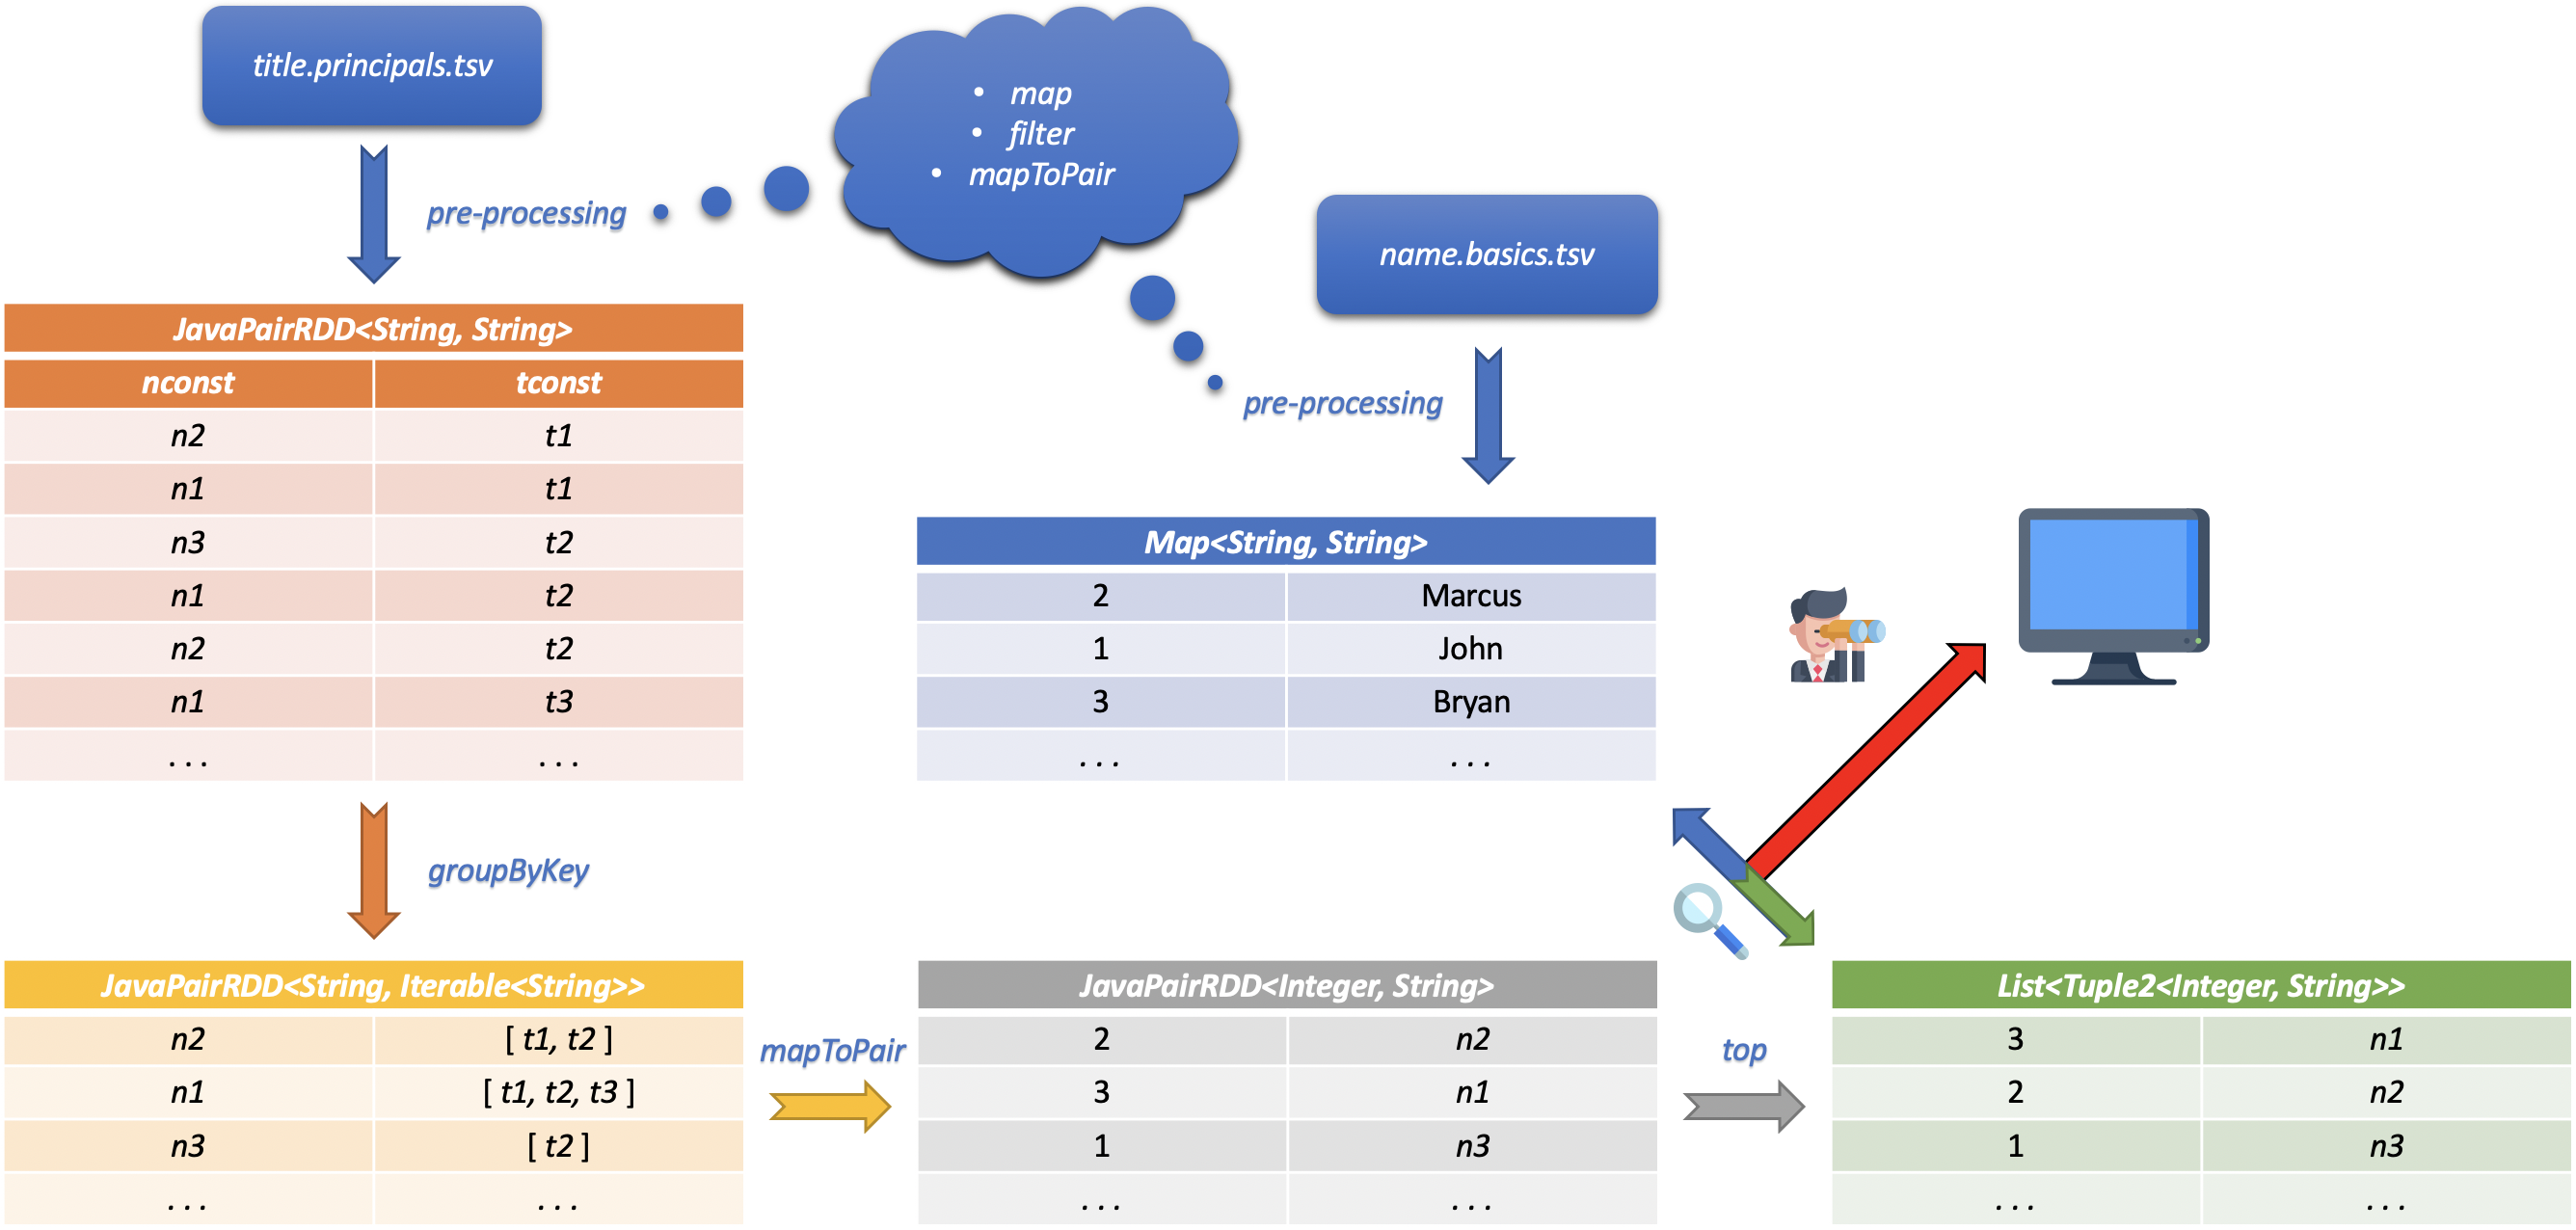
\includegraphics[width=1.0\textwidth]{Imagens/2ª Tarefa - Top10.png}
                \caption{2ª Tarefa (\textit{batch}) - Esquema do processamento relativo à subtarefa \textit{Top10}}
                \label{fig:17}
            \end{figure}

            \subsubsection{Alternativa} \label{sssec:Task2-Top10-Alternativa}
                Uma forma alternativa de resolver este exercício seria, na última fase do processamento, utilizar o método \textit{take} em detrimento da função \textit{top}.
                Esta escolha não foi tomada em consideração na implementação uma vez que o primeiro método necessita previamente que a informação esteja devidamente ordenada.
                Esta ordenação teria de ser realizada com a invocação do método \textit{sortByKey(false)}, colocando a contagem dos filmes em que cada ator participou de forma decrescente.
                Este último facto representa uma ineficiência no cálculo do resultado pretendido uma vez que é efetuada a ordenação completa da informação em causa e, para além disso, realiza-se desnecessariamente um passo computacional extra.

        \subsection{\textit{Friends}} \label{subsec:Task2-Friends}
            Neste exercício é requerido a computação do conjunto de colaboradores associado a cada ator, ou seja, o grupo dos atores que particapam nos mesmos filmes.
                
            Durante o processamento inicial do ficheiro \textsl{"title.principals.tsv"} é, tal como seria de esperar, ignorado o respetivo cabeçalho.
            Posteriormente, é extraída, linha após linha, a informação pertinente do mesmo, isto é, os identificadores do filme e do ator em questão, agrupando os dados pela primeira componente. Esta última ação é efetuada com recurso à chamada do método \textit{groupByKey}.
            De forma a obter o resultado solicitado nesta subtarefa, é necessário, nesta fase da computação, proceder à realização de uma operação denominada por produto cartesiano. Nesta operação computa-se, num dado momento, vários pares de atores que coloboraram num determinado filme.
            Uma vez realizado este cálculo, é invocado novamente o método \textit{groupByKey} de forma a obter o resultado pretendido, isto é, o conjunto de colaboradores para cada ator presente nos dados públicos do \textit{IMDb}.

            \begin{figure}[H]
                \centering
                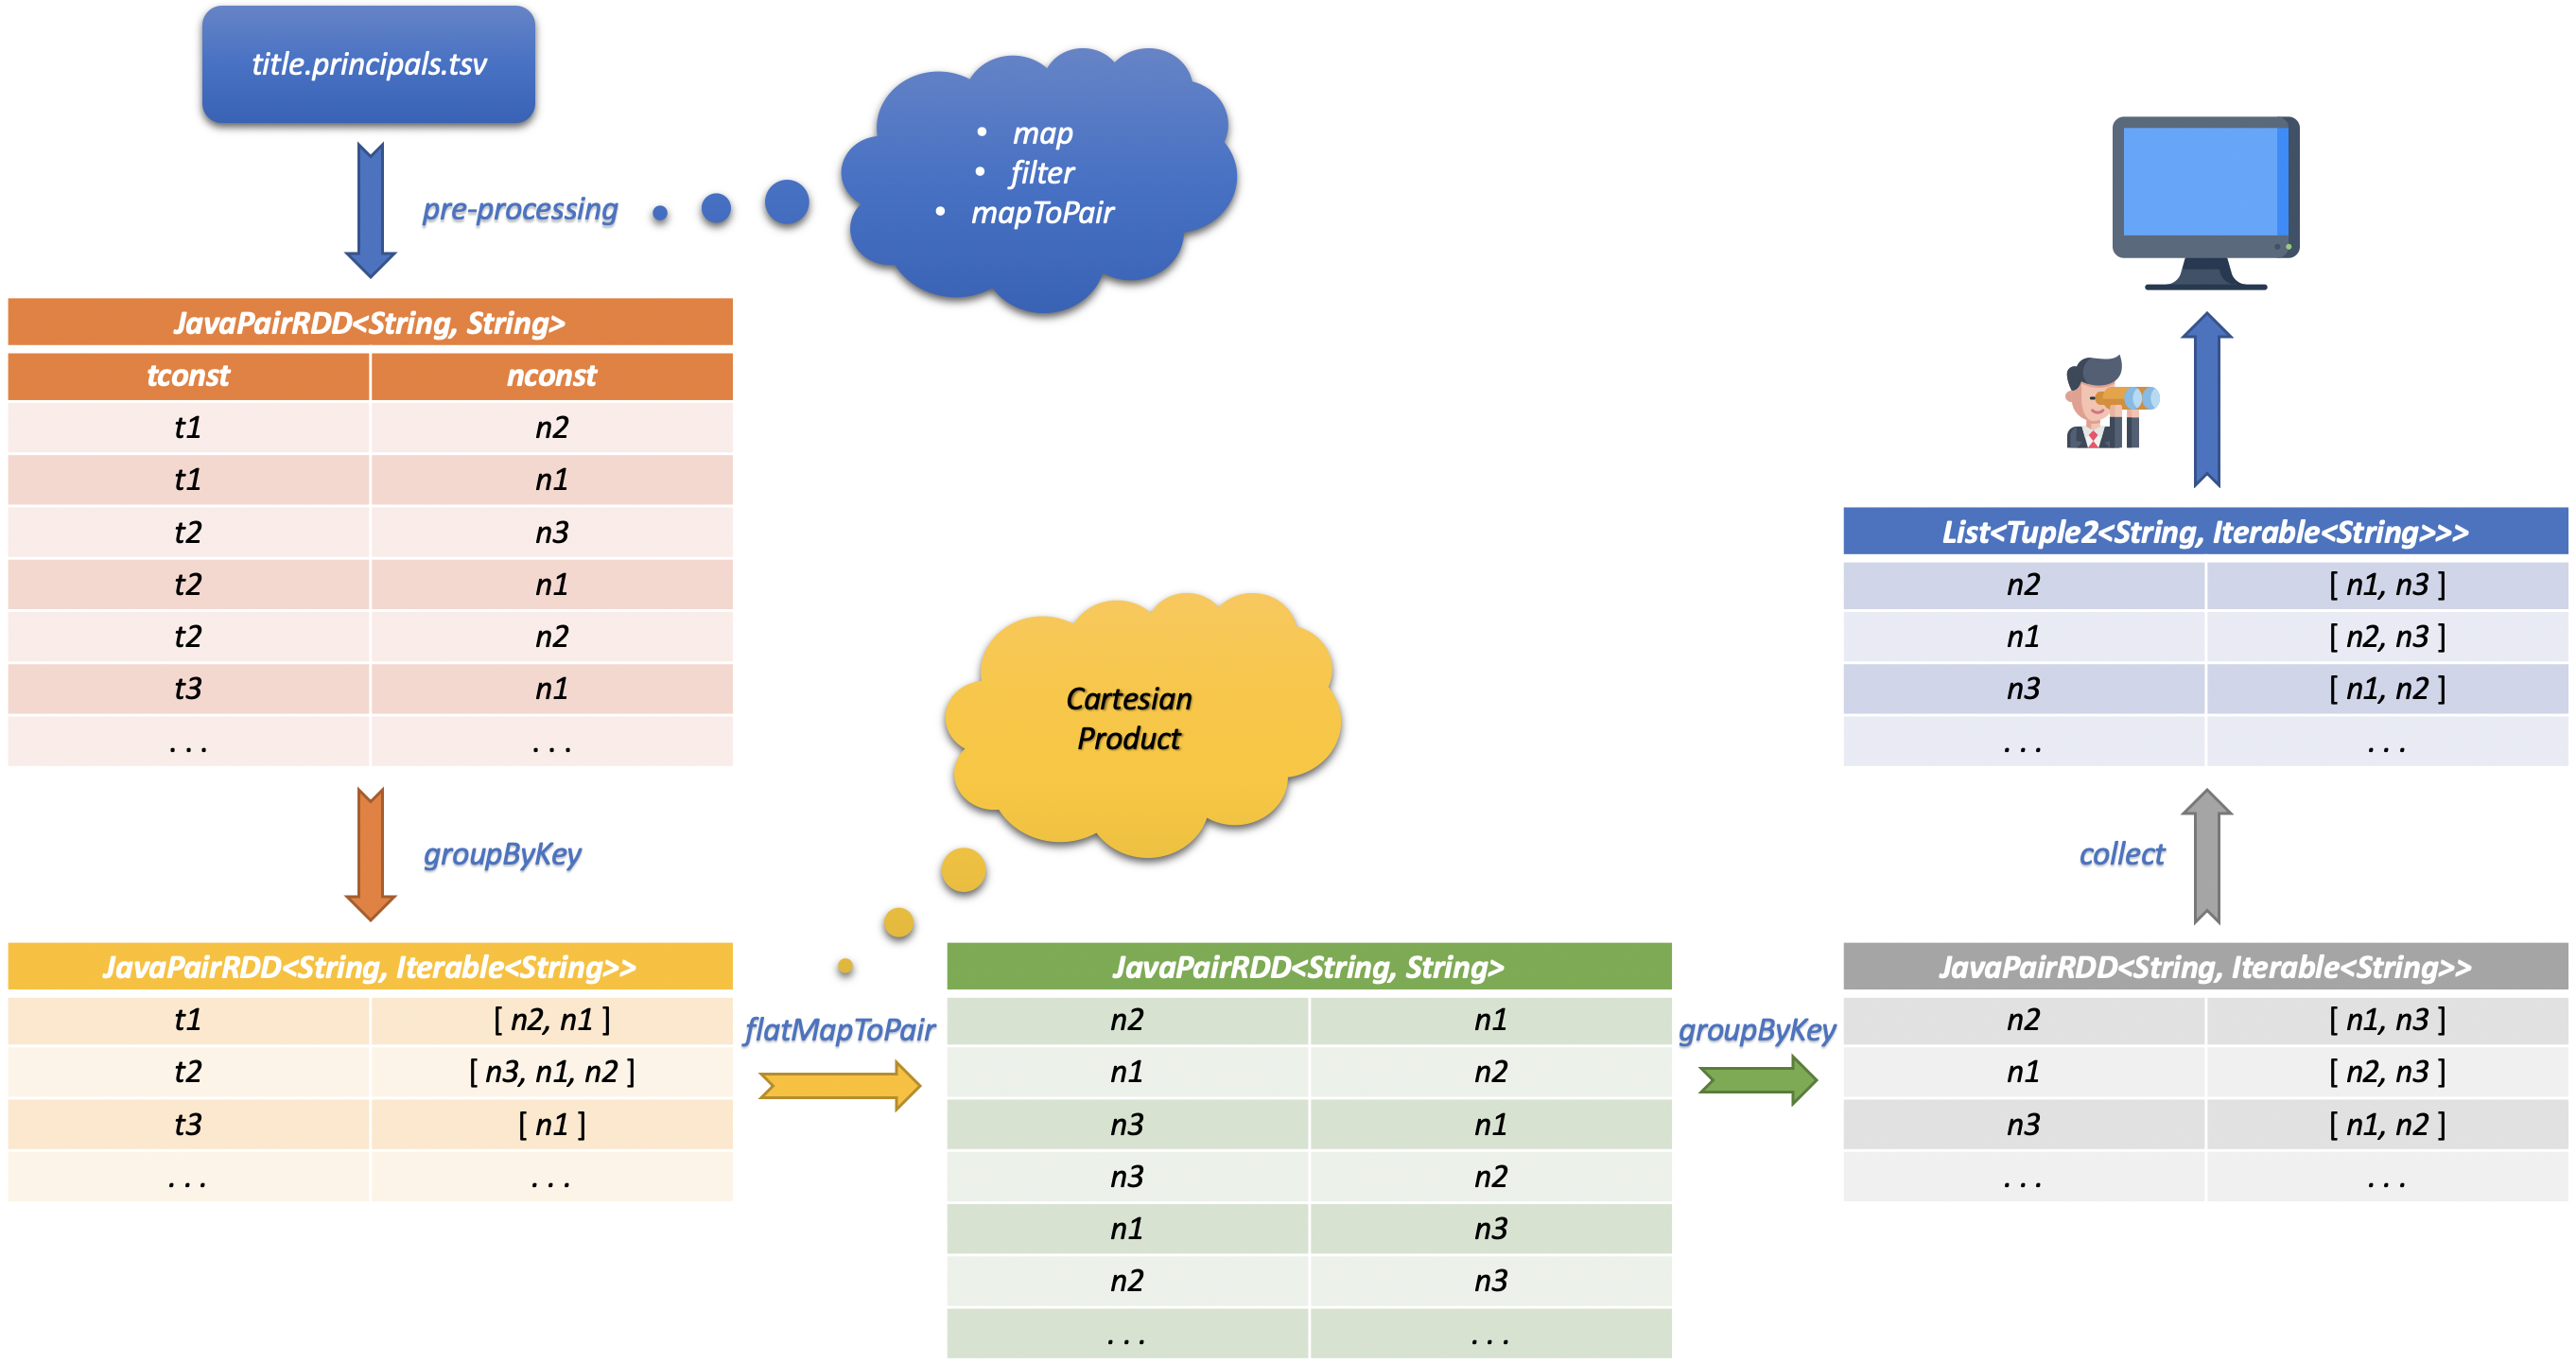
\includegraphics[width=1.0\textwidth]{Imagens/2ª Tarefa - Friends.png}
                \caption{2ª Tarefa (\textit{batch}) - Esquema do processamento relativo à subtarefa \textit{Friends}}
                \label{fig:18}
            \end{figure}

            \subsubsection{Alternativa} \label{sssec:Task2-Friends-Alternativa}

        \subsection{\textit{Ratings}} \label{subsec:Task2-Ratings}
            \subsubsection{Alternativa} \label{sssec:Task2-Ratings-Alternativa}

    \section{3ª Tarefa} \label{sec:Task3}


\chapter{Conclusão} \label{ch:Conclusion}
\large{
    
}

\appendix
\chapter{Observações} \label{ch:Observations}
\begin{itemize}
    \item Documentação \textit{Java} 8:
    \par \textit{\url{https://docs.oracle.com/javase/8/docs/api/}}
    \item \textit{Maven}:
    \par \textit{\url{https://maven.apache.org/}}
    \item \textit{Docker}:
    \par \textit{\url{https://www.docker.com/}}
    \item \textit{Apache Spark}:
    \par \textit{\url{https://spark.apache.org/}}
    \item \textit{Apache Hadoop}:
    \par \textit{\url{http://hadoop.apache.org/}}
\end{itemize}

\end{document}